\section{Improved Client GUI}
Inspired by the recently completed World Chess Championship and our group name, IPM (abbreviation of Introductory Programming, group M), being a pun on IBM. We decided to implement a visual style honouring the late, great chess computer, Deep Blue.

The site has a simple mobile-first layout. A dynamic background resembling the inner workings of a sophisticated AI fills the screen. In front are simple form elements with a retro, monospace font (Figure \ref{fig:gui:noResults}). A search is carried out both when clicking on the search button and when pressing \textit{Enter} while focus is in the search field. When a search has been completed, a few details are displayed: The amount of websites retrieved, the time it took, and a tip of the hat to Garry Kasparov. Below, results are displayed with a simple preview (Figure \ref{fig:gui:results}). 

\begin{figure}
	\centering
	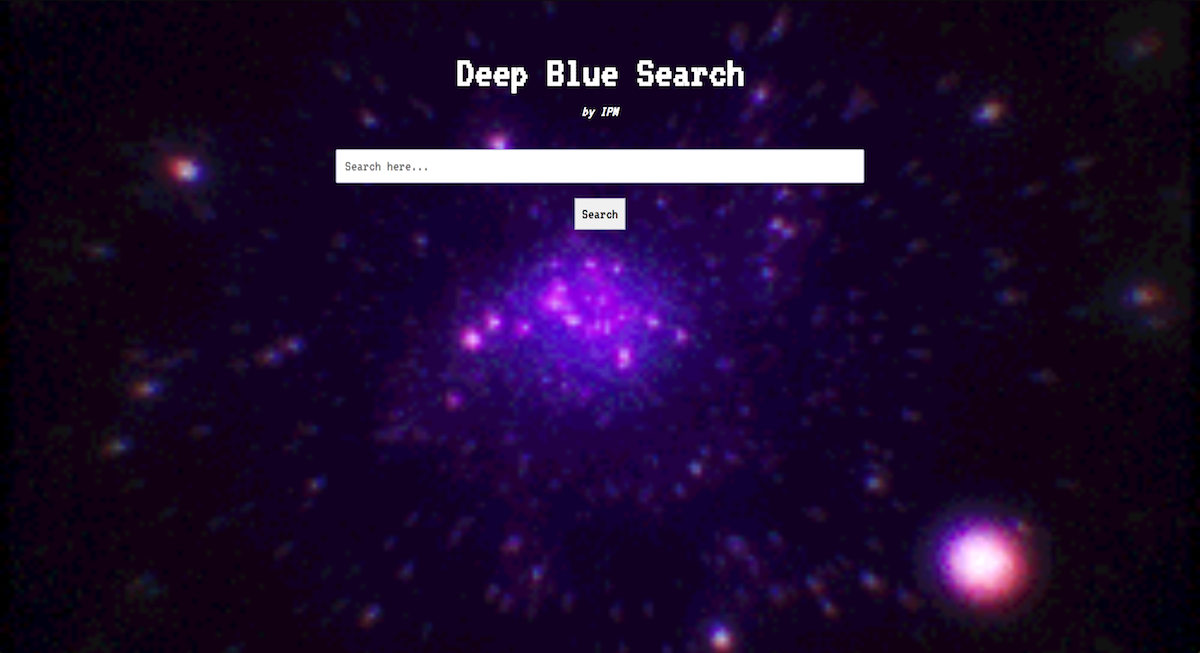
\includegraphics[width=\textwidth]{graphics/gui-noResults.png}
	\caption{The GUI before a search is conducted.}
	\label{fig:gui:noResults}
\end{figure}

\begin{figure}
	\centering
	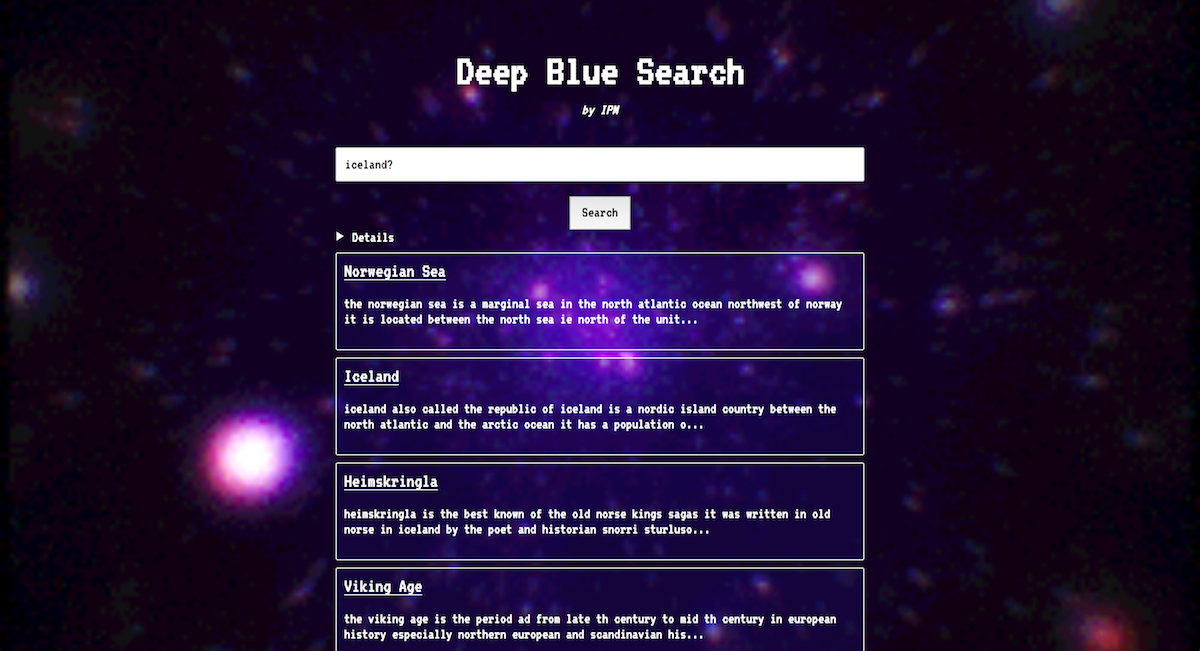
\includegraphics[width=\textwidth]{graphics/gui.png}
	\caption{The GUI after a search has been conducted.}
	\label{fig:gui:results}
\end{figure}